\documentclass{article}
\usepackage{latexsym}
\usepackage{graphicx}
\usepackage{url}
\usepackage{hyperref}
\usepackage{listings}
\hypersetup{colorlinks=true}


\begin{document}



\title{Bloom filter, Summer 2017}
\author{Minoiu George Emilian}
\date{\today}
\maketitle

\begin{tabbing}
\\ \\ \\ \\ \\ \\ \\ \\ \\ \\ \\ \\ \\ \\ \\ \\ \\ \\ \\ \\ \\ \\ \\ \\
\end{tabbing}

\begin{tabbing}
\indent{Teacher:}  \=\ {Costin B\u{a}dic\u{a}} \\
\indent{Section:}   \=\  {Computers with teaching in Romanian Class} \\
\indent{Group:}      \>  C.R. 1.2.  \\
\indent{Year of study:} \=\ {I}

\end{tabbing}

\pagebreak
% sections
\section{Problem statement}
\ \ \ \ A library for bloom filters . The library should allow inserting and searching for an item.

\section{Pseudocode}
\begin{center}
\lstset{
  language=C,                % choose the language of the code
  numbers=left,                   % where to put the line-numbers
  stepnumber=1,                   % the step between two line-numbers.        
  numbersep=5pt,                  % how far the line-numbers are from the code
  backgroundcolor=\color{white},  % choose the background color. You must add \usepackage{color}
  showspaces=false,               % show spaces adding particular underscores
  showstringspaces=false,         % underline spaces within strings
  showtabs=false,                 % show tabs within strings adding particular underscores
  tabsize=4,                      % sets default tabsize to 2 spaces
  captionpos=b,                   % sets the caption-position to bottom
  breaklines=true,                % sets automatic line breaking
  breakatwhitespace=true,         % sets if automatic breaks should only happen at whitespace \lstinputlisting;
}

\begin{lstlisting}


int * quick_sort(struct Array *array){


    int size_array = size_of(array);
    int *aux = copy_array(array, size_array);
    int i;
    int j;
    int aux_number;
    int swap_number;
    begin_clock();

    quickSort(aux, 0, size_array-1);

    end_clock("Quick sort", 4);

    if(G_ACTIVATE_PRINT == 1){
        printf("\nArray after sorting: ");

        for(i = 0; i < size_array; i++)
            printf("%d ", aux[i]);
    }

    return aux;
}

void binary_search(struct Array *array, int number){

    int size_array = size_of(array);
    int *aux = sort_with_best(array, size_array);
    int aux_number;
    int left;
    int right;
    int middle;

    begin_clock();

    left = 0;
    right = size_array - 1;

    while (left <= right){
        middle = left + (right - left)/2;
        if (aux[middle] == number){
            printf("\nNumber %d found at position %d.", number, middle);
            break;
        }
        if (aux[middle] < number)
            left = middle + 1;
        else
            right = middle - 1;
    }

    if(left > right)
        printf("\nNumber %d was not found in the array.", number);

    end_clock("Binary search", 8);

}


\end{lstlisting}
\end{center}

\pagebreak

\subsection{Pseudocode description}
\textbf{}
\indent The {\bf quick sort} function is made for quick sorting a given array without modifying it. It's one of the methods used for sorting array from this program. \\
The {\bf binary\_search} function is sorting an array with the best method of sorting found so far than binary search an item in the sorted array. \\

\section{Application Design}
\subsection{Main}
\textbf{}
\indent The {\bf main} of my program contains a {\bf while} loop so the user will be forced to choose a valid option. The user has the option to choose from sixteen different options, including all types of sorting, adding a number to the end of our array, adding a number to the beginning of our array, generate random numbers.
\\
The user will have to insert some values in order for functions to be called.

\subsection{Input Data}
\textbf{}
\indent For my program, input data is "decision". An integer value for choosing an option in from the menu or telling how many numbers i want to be generated in array or telling which is the number i want to search for in current array.

\subsection{Output Data}
\textbf{}
\indent The data outputs resulted from functions processing. The functions include printing unmodified array to the console, printing array after sorting, printing the seconds that have passed for a sorting to be done, printing the seconds that have passed for a search to be done.




\pagebreak

\subsection{Functions used}
\textbf{}
\indent{\bf queue\_pointer new\_queue(int queue\_size)} function is used to allocate dynamically a new queue. It creates a new priority queue with the given size for it's elements. It returns the address of memory where our new priority queue starts.

{\bf int * bubble\_sort(struct Array *array)} function is used for an array to be bubble sorted. The seconds took for this operation are printed to the console.

{\bf int * insertion\_sort(struct Array *array)} function is used for an array to be insertion sorted. The seconds took for this operation are printed to the console.

{\bf int * selection\_sort(struct Array *array)} function is used for an array to be selection sorted. The seconds took for this operation are printed to the console.

{\bf int * quick\_sort(struct Array *array)} function is used for an array to be quick sorted. The seconds took for this operation are printed to the console.

{\bf int * merge\_sort(struct Array *array)} function is used for an array to be merge sorted. The seconds took for this operation are printed to the console.

{\bf int * heap\_sort(struct Array *array)} function is used for an array to be heap sorted. The seconds took for this operation are printed to the console.

{\bf int * radix\_sort(struct Array *array)} function is used for an array to be radix sorted. The seconds took for this operation are printed to the console.

{\bf int * radix\_sort(struct Array *array)} function is used for an array to be radix sorted. The seconds took for this operation are printed to the console.


{\bf int * sort\_with\_best(struct Array *array, int size)} function is used for an array to be sorted using the best method found so far. Sorting with all types of sorting will determine the best method. 

{\bf void binary\_search(struct Array *array, int number)} function is used to search for a number into the given array. The array is being sorted at first using the best method found so far after the number is being searched. 

{\bf void linear\_search(struct Array *array, int number)} function is used to search for a number into the given array. The search will be linear. 

{\bf begin\_clock()} function is used to start a clock at the beginning of each function. 


{\bf void end\_clock(char sorting\_method[100], unsigned int sorting\_number)} function is used to end the already started clock and prints result to the console. 





\section{Source code}
\textbf{}
\indent My program is wrote in C99 standard. It has basic libraries and functions

The code is compiled in two different compilers: "GNU GCC Compiler" and "Visual C++".


\pagebreak
\section{Experiments and results}
\subsection{GCC Compiler}
\textbf{}
\begin{center}
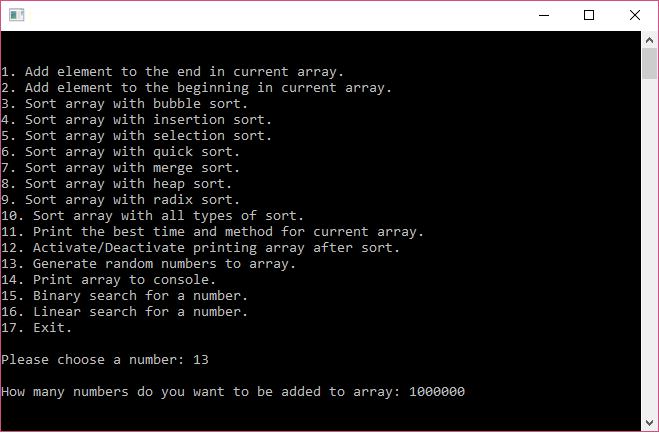
\includegraphics[scale=0.90]{c1.png} \\
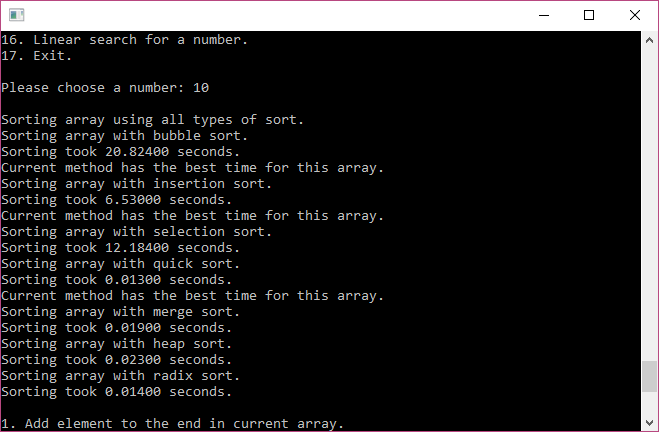
\includegraphics[scale=0.90]{c2.png} \\
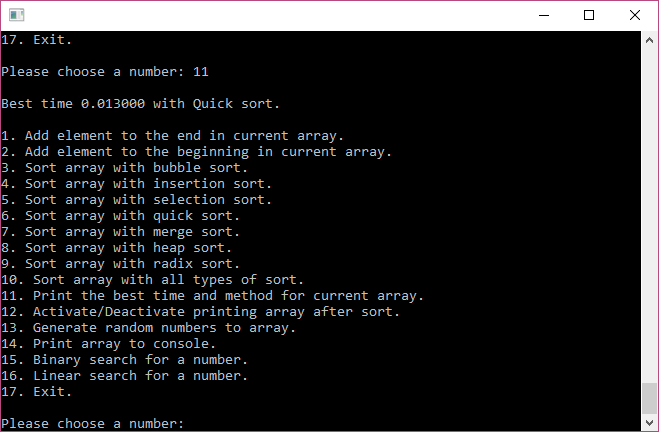
\includegraphics[scale=0.90]{c3.png} \\
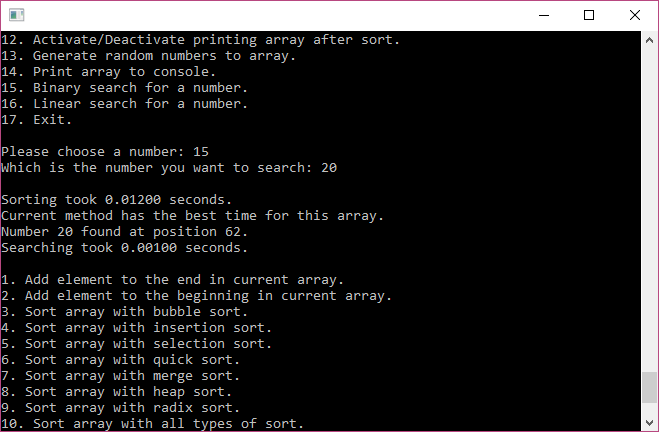
\includegraphics[scale=0.90]{c4.png} \\
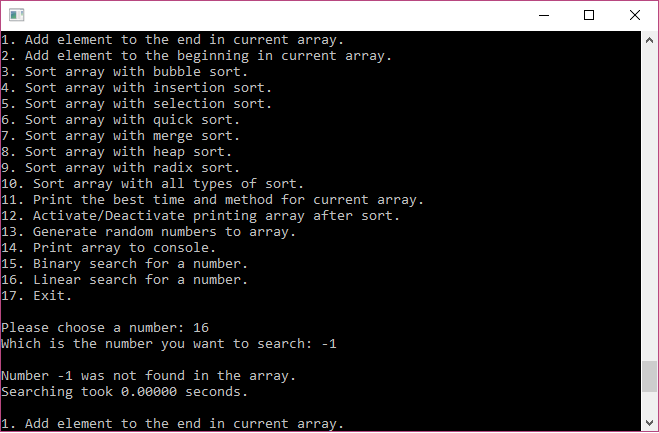
\includegraphics[scale=0.90]{c5.png} \\
\end{center}
\pagebreak


\section{Conclusions}
\textbf{}
\indent Dynamic allocation of memory is helping me store and generate numbers till my memory fills up.


% bibliography
\begin{thebibliography}{9}

	\bibitem{lk}
	 {\bf Links} \\
	 Alexander S. Kulikov, Singly linked lists \url{https://www.coursera.org/learn/data-structures/lecture/kHhgK/singly-linked-lists} \\
	 Neil Rhodes,University of California, San Diego \url{https://www.coursera.org/learn/data-structures/lecture/OsBSF/arrays}

\end{thebibliography}

\end{document}